%----------------------------------------------------------------------------------------
%	PACKAGES AND OTHER DOCUMENT CONFIGURATIONS
%----------------------------------------------------------------------------------------

\documentclass{article}

\usepackage{fancyhdr} % Required for custom headers
\usepackage{lastpage} % Required to determine the last page for the footer
\usepackage{extramarks} % Required for headers and footers
\usepackage{graphicx} % Required to insert images
\usepackage{amsmath, amssymb} % Required for Maths
\usepackage{mathtools} % Required for Maths
\usepackage{enumerate}

% Margins
\topmargin=-0.45in
\evensidemargin=0in
\oddsidemargin=0in
\textwidth=6.5in
\textheight=9.0in
\headsep=0.25in 

\linespread{1.1} % Line spacing

% Set up the header and footer
\pagestyle{fancy}
\lhead{\hmwkAuthorName} % Top left header
\chead{\hmwkClass\ (\hmwkClassInstructor\ \hmwkClassTime): \hmwkTitle} % Top center header
\rhead{\firstxmark} % Top right header
\lfoot{\lastxmark} % Bottom left footer
\cfoot{} % Bottom center footer
\rfoot{Page\ \thepage\ of\ \pageref{LastPage}} % Bottom right footer
\renewcommand\headrulewidth{0.4pt} % Size of the header rule
\renewcommand\footrulewidth{0.4pt} % Size of the footer rule

\setlength\parindent{0pt} % Removes all indentation from paragraphs

%----------------------------------------------------------------------------------------
%	DOCUMENT STRUCTURE COMMANDS
%	Skip this unless you know what you're doing
%----------------------------------------------------------------------------------------

% Header and footer for when a page split occurs within a problem environment
\newcommand{\enterProblemHeader}[1]{
\nobreak\extramarks{#1}{#1 continued on next page\ldots}\nobreak
\nobreak\extramarks{#1 (continued)}{#1 continued on next page\ldots}\nobreak
}

% Header and footer for when a page split occurs between problem environments
\newcommand{\exitProblemHeader}[1]{
\nobreak\extramarks{#1 (continued)}{#1 continued on next page\ldots}\nobreak
\nobreak\extramarks{#1}{}\nobreak
}

\setcounter{secnumdepth}{0} % Removes default section numbers
\newcounter{homeworkProblemCounter} % Creates a counter to keep track of the number of problems

\newcommand{\homeworkProblemName}{}
\newenvironment{homeworkProblem}[1][Problem \arabic{homeworkProblemCounter}]{ % Makes a new environment called homeworkProblem which takes 1 argument (custom name) but the default is "Problem #"
\stepcounter{homeworkProblemCounter} % Increase counter for number of problems
\renewcommand{\homeworkProblemName}{#1} % Assign \homeworkProblemName the name of the problem
\section{\homeworkProblemName} % Make a section in the document with the custom problem count
\enterProblemHeader{\homeworkProblemName} % Header and footer within the environment
}{
\exitProblemHeader{\homeworkProblemName} % Header and footer after the environment
}

\newcommand{\problemAnswer}[1]{ % Defines the problem answer command with the content as the only argument
\noindent\framebox[\columnwidth][c]{\begin{minipage}{0.98\columnwidth}#1\end{minipage}} % Makes the box around the problem answer and puts the content inside
}

\newcommand{\homeworkSectionName}{}
\newenvironment{homeworkSection}[1]{ % New environment for sections within homework problems, takes 1 argument - the name of the section
\renewcommand{\homeworkSectionName}{#1} % Assign \homeworkSectionName to the name of the section from the environment argument
\subsection{\homeworkSectionName} % Make a subsection with the custom name of the subsection
\enterProblemHeader{\homeworkProblemName\ [\homeworkSectionName]} % Header and footer within the environment
}{
\enterProblemHeader{\homeworkProblemName} % Header and footer after the environment
}

%----------------------------------------------------------------------------------------
%	NAME AND CLASS SECTION
%----------------------------------------------------------------------------------------

\newcommand{\hmwkTitle}{Homework\ \#1} % Assignment title
\newcommand{\hmwkDueDate}{Wednesday,\ September\ 16,\ 2015} % Due date
\newcommand{\hmwkClass}{ENPM 808M} % Course/class
\newcommand{\hmwkClassTime}{4:00 PM} % Class/lecture time
\newcommand{\hmwkClassInstructor}{Dr. William Levine} % Teacher/lecturer
\newcommand{\hmwkAuthorName}{Kanishka Ganguly} % Your name

%----------------------------------------------------------------------------------------
%	TITLE PAGE
%----------------------------------------------------------------------------------------

\title{
\vspace{2in}
\textmd{\textbf{\hmwkClass:\ \hmwkTitle}}\\
\normalsize\vspace{0.1in}\small{Due\ on\ \hmwkDueDate}\\
\vspace{0.1in}\large{\textit{\hmwkClassInstructor\ \hmwkClassTime}}
\vspace{3in}
}

\author{\textbf{\hmwkAuthorName}}
\date{} % Insert date here if you want it to appear below your name

%----------------------------------------------------------------------------------------

\begin{document}

\maketitle

%----------------------------------------------------------------------------------------
%	TABLE OF CONTENTS
%----------------------------------------------------------------------------------------

%\setcounter{tocdepth}{1} % Uncomment this line if you don't want subsections listed in the ToC

\newpage
\tableofcontents
\newpage

%----------------------------------------------------------------------------------------
%	PROBLEM 1
%----------------------------------------------------------------------------------------

% To have just one problem per page, simply put a \clearpage after each problem

\begin{homeworkProblem}
\vspace{10pt}
Consider the block sliding on a wedge from Lecture \#1. Suppose the block has mass \textit{$M_1$} and the wedge has mass \textit{$M_2$}. The angle of the block is \textit{$\alpha$} as in the lecture. When \textit{$M_1$} slides down and to the left, the wedge \textit{$M_2$} slides to the right. Find formulae for the acceleration of \textit{$M_1$} and \textit{$M_2$} in the absence of friction.

\problemAnswer{ % Answer
\begin{center}
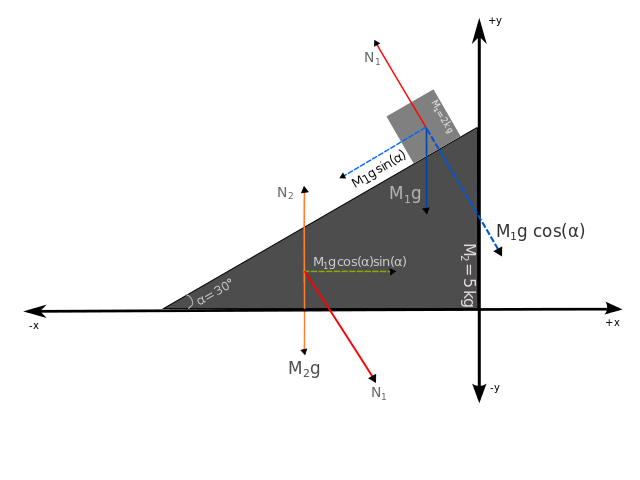
\includegraphics[width=0.75\columnwidth]{Q1.png} % Q1_Image
\end{center}
}
\vspace{20pt}
As can be seen from the figure, we have the free body diagram of the wedge and block system. \\
The block slides along the wedge with an acceleration in the $x$ and $y$ directions while the wedge has only an acceleration along the $x$-axis.\\
Now, consider the forces on the block only. We have a downward force of $M_1g$ perpendicular to the reference frame, which is the force due to the acceleration due to gravity. We also have a normal reaction of force $N_1$ caused due to the contact forces between the block and the wedge. If we resolve these forces into their horizontal and vertical components, we have: \\
\begin{align}
(F_1)_\parallel = M_1 \times g \times cos(\alpha)\\
(F_1)_\perp = M_1 \times g \times sin(\alpha)\\
(N_1)_\perp = N_1 \times sin(\alpha)
\end{align}\newline

Now, consider the forces on the wedge only. We have a downward force of $M_2g$ perpendicular to the reference frame, which is the force due to the acceleration due to gravity. We also have a normal reaction of force $N_2$ caused due to the contact forces between the wedge and the ground. \newline

Now, consider the system of block and wedge together. It is assumed that there is negligible force due to friction. As a result, the wedge moves in the right direction due to the horizontal component of the downward force being applied by the block, which is sliding to the right.\\
The forces $N_2$ and $M_2 g$ are equal and acting in opposite directions, hence there is no vertical motion of the wedge. There is only the horizontal component of force $N_1$ from the block acting on the wedge.
We have:
\begin{align}
N_1 = M_1 \times g \times cos(\alpha) \label{eq:N1}
\end{align}
and the horizontal component of Equation \ref{eq:N1} as:
\begin{align}
(N_1)_\parallel = M_1\times g \times cos(\alpha) \times sin(\alpha) \label{eq:horizontalwedge}
\end{align}\newline

From Newton's Second Law of Motion, we have:
\begin{align}
F = M\times a \\
\implies a = \frac{F} M \label{eq:accel}
\end{align} where $a$ is the acceleration, $F$ is the force applied, $M$ is the mass of the object. \\

So, from Equation \ref{eq:accel}, we calculate the force and the resulting acceleration on the wedge as follows:\\
\begin{align}
N_2 = Ncos(\theta) - Nsin(\theta)\\
N_2sin(\theta) = M_2\times A\\
\implies A = \frac{Nsin(\theta)}{M_2}
\end{align}\\

So, from Equation \ref{eq:accel}, we calculate the force and the resulting acceleration on the block as follows:\\\\
Along the vertical direction,
\begin{align}
M_1\times g - N_1 \times cos(\theta) = M_1 \times sin(\theta)\\
M_1\times g - \Big( \frac{{M_2\times A}}{sin(\theta)} \Big) = M_1\times a \times sin(\theta)\\
M_1\times g \times sin(\theta) - M_2 \times A \times cos(\theta) = M_1 \times a \times sin^2(\theta) \label{eq:finda}
\end{align}
\\\\
Along the horizontal direction,
\begin{align}
N_1 \times sin(\theta) = M_1 \times (a\times cos(\theta) - A)\\
N_1 \times sin(\theta) + M_1 \times A = M_1 \times a \times cos(\theta)\\
\Big( \frac{M_2\times A}{sin(\theta)} \Big) \times sin(\theta) + M_1A = M_1acos(\theta)\\
A(M_2 + M_1) = M_1acos(\theta)\\
\implies A = \frac{M_1acos(\theta)}{(M_1+M_2)} \label{eq:A}
\end{align}
\\\\
Substituting $A$ from Eqn.\ref{eq:A} in Eqn.\ref{eq:finda}, we have\\
\begin{align}
M_1gsin(\theta) - M_2\Big(\frac{M_1acos(\theta)}{M_1+M_2} \Big) \times cos(\theta) = M_1asin^2(\theta)\\
M_1(M_1 + M_2)gsin(\theta) - M_1M_2acos^2(\theta) = M_1(M_1 + M_2)asin^2(\theta)\\
(M_1+M_2)gsin(\theta) = M_1asin^2(\theta) + M_2asin^2(\theta) + M_2acos^2(\theta)\\
(M_1 + M_2)gsin(\theta) = M_1asin^2(\theta) + M_2a\\
\implies a = \frac{(M_1+M_2)gsin(\theta)}{M_1sin^2(\theta) + M_2} \label{eq:a}
\end{align}
\\\\
Thus, from Eqn.\ref{eq:a} we have the acceleration of the block as:\\
\begin{align}
\mathbf{a = \frac{7\times 9.8 \times 0.5}{(2\times 0.25) + 5} = 6.23 m/s^2}\\
\end{align}
So, taking the components of this acceleration, we have
\begin{align}
\mathbf{a_x = 6.23 \times cos(30) = 5.390 m/s^2}\\
\mathbf{a_y = 6.23 \times sin(30) = 3.115 m/s^2}
\end{align}\\
Thus, from Eqn.\ref{eq:A} we have the acceleration of the wedge as:\\
\begin{align}
\mathbf{A_x = \frac{(2\times 6.23 \times cos(30))}{2 + 5}}\\
\mathbf{A_x = 1.530 m/s^2}
\end{align}


\end{homeworkProblem}
\clearpage

%----------------------------------------------------------------------------------------
%	PROBLEM 2
%----------------------------------------------------------------------------------------

\begin{homeworkProblem} % Custom section title
 A 5 kilogram weight hangs from a spring of such stiffness that the spring stretches $\delta = 1 cm$  under the weight.
\begin{enumerate}[a.]	
\item Calculate the stiffness of the spring.
\item Calculate the natural frequency of the up and down oscillations of the weight if it starts at some length other than stretched by $\delta = 1 cm$.
\item Write a formula for the frequency in terms of $\delta$ alone, in which neither the mass $m$ nor the spring constant $k$ appears.
\end{enumerate}
%--------------------------------------------

\begin{homeworkSection}{(a)} % Section within problem
\vspace{10pt} % Question
\problemAnswer{ % Answer

\begin{center}
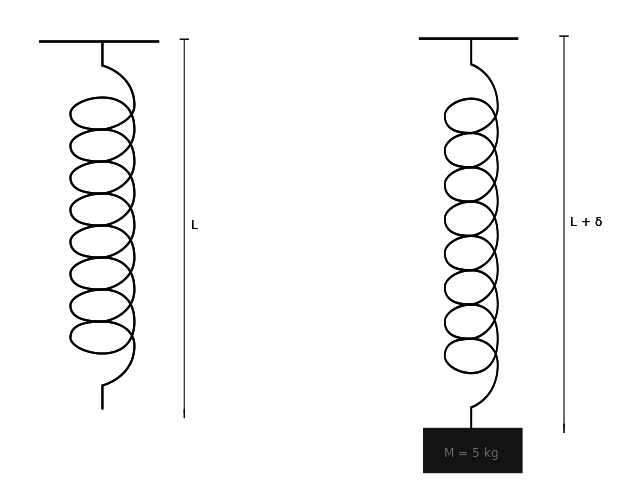
\includegraphics[width=0.65\columnwidth]{Q2.png} \label{fig:Q2}% Q2_Image
\end{center}
\vspace{10pt}

As can be seen in above figure, we have a spring of length $L$ when it is in its natural position, without any external mass attached to it. Once a mass $M$ of 5 kg is attached to the end of the spring, there is a change in length of $\delta = 1 cm$.\\
Now, we know from Hooke's Law that \textit{the force needed to extend or compress a spring by some distance is proportional to that distance.}\\
Or, formally, we have 
\begin{align}
F = -k \times \delta \label{eq:hooke}
\end{align}
where $k$ is the spring constant, or a characteristic value of the spring denoting its stiffness.\\

So, from Equation \ref{eq:hooke}, we have:
\begin{align}
F = -k \times \delta\\
\implies k = \frac{-F}\delta\\
\implies k = \frac{5 \times 9.8} {0.01} = 4900 \text{N/m}
\end{align}
}

\end{homeworkSection}

%--------------------------------------------

\begin{homeworkSection}{(b)} % Section within problem
\problemAnswer{ % Answer
Continuing with figure shown previously, the formula for the frequency of oscillations of the weight $M$ attached to the spring when released from a length other than $\delta$ is:
\begin{align}
\omega = \frac{1}{2\pi}\sqrt{\frac{k}{M}} \label{eq:frequency}
\end{align}
where $\omega$ is the frequency of oscillation, $k$ is the spring constant of the spring and $M$ is the mass of the weight attached to the spring.\newline

So, from Equation \ref{eq:frequency}, we have:
\begin{align}
\omega = \frac{1}{2\pi}\sqrt{\frac{4900}{5}}\\
\implies \omega = \frac{1}{2\pi}\sqrt{980}\\ 
\implies \mathbf{\omega = 4.98 s^{-1}}
\end{align}
}
\end{homeworkSection}

%--------------------------------------------

\begin{homeworkSection}{(c)} % Section within problem
\problemAnswer{ % Answer
Continuing with figure shown previously, the formula for the frequency of oscillations of the weight $M$ attached to the spring when released from a length other than $\delta$ is:
\begin{align}
\omega = \frac{1}{2\pi}\sqrt{\frac{k}{M}} \label{eq:frequency2}
\end{align}
where $\omega$ is the frequency of oscillation, $k$ is the spring constant of the spring and $M$ is the mass of the weight attached to the spring.\newline

Also, we know that:
\begin{align}
k = \frac{M \times g}{\delta} \label{eq:k}
\end{align}

So, from Equation \ref{eq:frequency2} and \ref{eq:k}, we have:
\begin{align}
\omega = \frac{1}{2\pi}\sqrt{\frac{\frac{M \times g}{\delta}}{M}}
\end{align}
Simplifying, we have:
\begin{align}
\mathbf{\omega = \frac{1}{2\pi}\sqrt{\frac{g}{\delta}}}\label{eq:withoutTerms}
\end{align}

where $g$ is the acceleration due to gravity and $\delta$ is the displacement of the spring when a weight is attached to it. As can be seen, Equation \ref{eq:withoutTerms} does not contain any terms containing the mass $M$ or the spring constant $k$.
}
\end{homeworkSection}

%--------------------------------------------

\end{homeworkProblem}
\clearpage

%----------------------------------------------------------------------------------------
%	PROBLEM 3
%----------------------------------------------------------------------------------------

\begin{homeworkProblem}
A wheel has initial angular velocity 500 rpm and is being slowed down at a rate of 2 rpm per
second. How many rotations does the wheel make before it comes to a stop?
\begin{center}
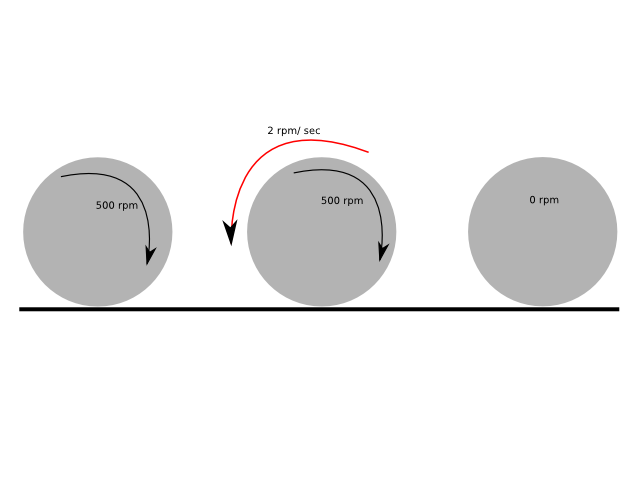
\includegraphics[width=1\columnwidth]{Q3.png} \label{fig:Q3}% Q3_Image
\end{center}
%--------------------------------------------
\problemAnswer{ % Answer


From the figure, we have the wheel rotating at an angular velocity $\omega = 500 rpm$. There is a retardation of 2 rpm per second.\\
We have the following formula for angular motion:
\begin{align}
\theta = (\omega_0 \times t) + \Big(\frac{1}2 \times \alpha \times t^2 \Big) \label{eq:motion}\\
\omega = \omega_0 + \alpha \times t \label{eq:motion2 }
\end{align}
where $\theta$ is the angular displacement of the wheel, $\omega_0$ is the initial angular velocity of the wheel, $\omega$ is the final velocity of the wheel and $\alpha$ is the angular acceleration of the wheel and $t$ is the time.\newline

So, we have:
\begin{align}
\omega_0 = 500 rpm = \frac{500}{60} r/s = 8.333 r/s\\
\alpha =\textit{2 rev. per minute per second} = 0.03 r/{s^{2}}\\
\end{align}
From Equation \ref{eq:motion2 } we have:
\begin{align}
0 = 500 - 2 \times t\\
\implies t = 250 s \label{eqn:time}
\end{align}

Using Equations \ref{eq:motion} and \ref{eqn:time},
\begin{align}
\theta = (8.333 \times 250) + \Big(\frac{1}2 \times 0.03 \times 250^2  \Big)\\
\implies \theta = \frac{62500}{60} = \textbf{1041.667 revolutions}
\end{align}\newline
Thus, the wheel takes \textbf{1041.667 revolutions} to come to a stop.
}
%--------------------------------------------
\end{homeworkProblem}
\clearpage
\end{document}
